\StartChapterOnNewColumn{Anhang}
% Im Anhang keine zusaetzlichen Umbruch-Reserven: dichter Satz.
\renewcommand{\BreakIfNotEnoughSpace}{}
\allowdisplaybreaks[4]

\SubsectionBar*{Anhang 1 -- Integraltabelle}
\begin{valuegridfive}
    & $\int_{0}^{\pi/4}$ & $\int_{0}^{\pi/2}$ & $\int_{0}^{\pi}$ & $\int_{0}^{2\pi}$ & $\int_{-\pi/2}^{\pi/2}$ \\
    $\sin x$ & $\frac{\sqrt{2}-1}{\sqrt{2}}$ & $1$ & $2$ & $0$ & $0$ \\
    $\sin^2x$ & $\frac{\pi-2}{8}$ & $\frac{\pi}{4}$ & $\frac{\pi}{2}$ & $\pi$ & $\frac{\pi}{2}$ \\
    $\sin^3x$ & $\frac{8-5\sqrt{2}}{12}$ & $\frac{2}{3}$ & $\frac{4}{3}$ & $0$ & $0$ \\
    $\cos x$ & $\frac{\sqrt{2}}{2}$ & $1$ & $0$ & $0$ & $2$ \\
    $\cos^2x$ & $\frac{2+\pi}{8}$ & $\frac{\pi}{4}$ & $\frac{\pi}{2}$ & $\pi$ & $\frac{\pi}{2}$ \\
    $\cos^3x$ & $\frac{5}{6\sqrt{2}}$ & $\frac{2}{3}$ & $0$ & $0$ & $\frac{4}{3}$ \\
    $\sin x\cos x$ & $\frac{1}{4}$ & $\frac{1}{2}$ & $0$ & $0$ & $0$ \\
    $\sin^2x\cos x$ & $\frac{1}{6\sqrt{2}}$ & $\frac{1}{3}$ & $0$ & $0$ & $\frac{2}{3}$ \\
    $\sin x\cos^2x$ & $\frac{4-\sqrt{2}}{12}$ & $\frac{1}{3}$ & $\frac{2}{3}$ & $0$ & $0$ \\
    $\sin^2x\cos^2x$ & $\frac{\pi}{32}$ & $\frac{\pi}{16}$ & $\frac{\pi}{8}$ & $\frac{\pi}{4}$ & $\frac{\pi}{8}$ \\
\end{valuegridfive}

\SubsectionBar*{Anhang 2 -- Integrale \ZSFScriptRef{72}}
\begin{formulabox}[breakable]
    \[
    \int x^n\,dx = \frac{1}{n+1}x^{n+1}+C
    \]
    \[
    \int \frac{1}{x^n}\,dx = -\frac{1}{n-1}\cdot\frac{1}{x^{n-1}}+C
    \]
    \[
    \int g'(\textcolor{cyan}{a}x+\textcolor{green!60!black}{b})\,dx = \frac{1}{\textcolor{cyan}{a}}\,g(\textcolor{cyan}{a}x+\textcolor{green!60!black}{b})+C
    \]
    \[
    \int \frac{f'(x)}{f(x)}\,dx = \ln(|f(x)|)+C
    \]
    \[
    \int \frac{1}{\textcolor{cyan}{a}x+\textcolor{green!60!black}{b}}\,dx = \frac{1}{\textcolor{cyan}{a}}\ln(|\textcolor{cyan}{a}x+\textcolor{green!60!black}{b}|)+C
    \]
    \[
    \int \frac{1}{(x-\textcolor{cyan}{a})(x-\textcolor{green!60!black}{b})}\,dx
    = \frac{1}{\textcolor{cyan}{a}-\textcolor{green!60!black}{b}}
    \ln\!\left(\left|\frac{x-\textcolor{cyan}{a}}{x-\textcolor{green!60!black}{b}}\right|\right)+C
    \]
    \[
    \int \frac{1}{\textcolor{cyan}{a}^2+x^2}\,dx = \frac{1}{\textcolor{cyan}{a}}\arctan\!\left(\frac{x}{\textcolor{cyan}{a}}\right)+C
    \]
    \[
    \int \frac{x}{\textcolor{cyan}{a}x^2+\textcolor{green!60!black}{b}}\,dx = \frac{1}{2\textcolor{cyan}{a}}\ln(|\textcolor{cyan}{a}x^2+\textcolor{green!60!black}{b}|)+C
    \]
    \[
    \int \frac{1}{1+x^2}\,dx = \arctan(x)+C
    \]
    \[
    \int \frac{x}{x^4+3}\,dx = \frac{\sqrt{3}}{6}\arctan\!\left(\frac{x^2}{\sqrt{3}}\right)+C
    \]
    \[
    \int \frac{1}{x^3+x}\,dx = \ln(|x|)-\frac{1}{2}\ln(x^2+1)+C
    \]
    \[
    \int \frac{1}{x^2+x}\,dx = \ln(|x|)-\ln(|x+1|)+C
    \]
    \[
    \int \frac{1}{1-x^2}\,dx = \mathrm{Artanh}(x)+C
    \]
\end{formulabox}

\begin{formulabox}[breakable]
    \textVorFormel{Wurzeln}
    \[
    \int \sqrt{x\pm \textcolor{cyan}{a}}\,dx = \frac{2}{3}(x\pm \textcolor{cyan}{a})^{3/2}+C
    \]
    \[
    \int \sqrt{1-x^2}\,dx = \frac{1}{2}\bigl(\arcsin(x)+x\sqrt{1-x^2}\bigr)+C
    \]
    \[
    \int \sqrt{\textcolor{cyan}{a}^2-x^2}\,dx = \frac{1}{2}\textcolor{cyan}{a}^2\arcsin\!\left(\frac{x}{\textcolor{cyan}{a}}\right) + \frac{1}{2}x\sqrt{\textcolor{cyan}{a}^2-x^2}+C
    \]
    \[
    \int 2x\sqrt{\textcolor{cyan}{a}+x^2}\,dx = \frac{2}{3}(\textcolor{cyan}{a}+x^2)^{3/2}+C
    \]
    \[
    \int \sqrt{x^2+1}\,dx = \frac{1}{2}\bigl(\mathrm{Arsinh}(x)+x\sqrt{1+x^2}\bigr)+C
    \]
    \[
    \int \frac{1}{\sqrt{1-x^2}}\,dx = \arcsin(x)+C=-\arccos(x)+C
    \]
    \[
    \int \frac{1}{\sqrt{x^2-1}}\,dx = \mathrm{arcosh}(x)+C
    \]
    \[
    \int \frac{x}{\sqrt{x^2-1}}\,dx = \sqrt{x^2-1}+C
    \]
    \[
    \int \frac{1}{\sqrt{x^2+1}}\,dx = \mathrm{Arsinh}(x)+C
    \]
    \[
    \int \frac{x}{\sqrt{1-x^2}}\,dx = -\sqrt{1-x^2}+C
    \]
    \[
    \int \frac{1}{\sqrt{x^2-4}}\,dx = \ln\!\left(\left|x+\sqrt{x^2-4}\right|\right)+C
    \]
\end{formulabox}

\begin{formulabox}[breakable]
    \textVorFormel{Exponential- und Logarithmusfunktionen}
    \[
    \int \frac{1}{x}\,dx = \ln(|x|)+C
    \]
    \[
    \int e^{\textcolor{cyan}{a}x}\,dx = \frac{1}{\textcolor{cyan}{a}}e^{\textcolor{cyan}{a}x}+C
    \]
    \[
    \int x e^x\,dx = (x-1)e^x+C
    \]
    \[
    \int x e^{x^2}\,dx = \frac{1}{2}e^{x^2}+C
    \]
    \[
    \int (x+1)e^x\,dx = x e^x+C
    \]
    \[
    \int \frac{1}{\sqrt{e^x-1}}\,dx = 2\arctan\!\bigl(\sqrt{e^x-1}\bigr)+C
    \]
    \[
    \int \ln(x)\,dx = x(\ln(|x|)-1)+C
    \]
    \[
    \int x\ln(x)\,dx = \frac{x^2\ln(|x|)}{2}-\frac{x^2}{4}+C
    \]
    \[
    \int \frac{(\ln(x))^n}{x}\,dx = \frac{(\ln(x))^{n+1}}{n+1}+C
    \]
    \[
    \int \frac{1}{x\ln(x)}\,dx = \ln(\ln(|x|))+C
    \]
\end{formulabox}

\begin{formulabox}[breakable]
    \textVorFormel{Trigonometrische Funktionen}
    \[
    \int \sin(\textcolor{cyan}{a}x)\,dx = -\frac{1}{\textcolor{cyan}{a}}\cos(\textcolor{cyan}{a}x)+C
    \]
    \[
    \int \cos(\textcolor{cyan}{a}x)\,dx = \frac{1}{\textcolor{cyan}{a}}\sin(\textcolor{cyan}{a}x)+C
    \]
    \[
    \int \tan(x)\,dx = -\ln(\cos(x))+C
    \]
    \[
    \int \frac{1}{\sin(x)}\,dx = \ln\!\left(\left|\frac{1-\cos(x)}{\sin(x)}\right|\right)+C
    \]
    \[
    \int \frac{1}{\cos(x)}\,dx = \ln\!\left(\left|\frac{1+\sin(x)}{\cos(x)}\right|\right)+C
    \]
    \[
    \int \cos^2(\textcolor{cyan}{a}x)\,dx = \frac{1}{2}\left(x+\frac{\sin(\textcolor{cyan}{a}x)\cos(\textcolor{cyan}{a}x)}{\textcolor{cyan}{a}}\right)+C
    \]
    \[
    \int \sin^2(\textcolor{cyan}{a}x)\,dx = \frac{1}{2}\left(x-\frac{\sin(\textcolor{cyan}{a}x)\cos(\textcolor{cyan}{a}x)}{\textcolor{cyan}{a}}\right)+C
    \]
    \[
    \int \sin(x)\cos^n(x)\,dx = -\frac{1}{n+1}\cos^{n+1}(x)+C
    \]
    \[
    \int \sin^n(x)\cos(x)\,dx = \frac{1}{n+1}\sin^{n+1}(x)+C
    \]
    \[
    \int \frac{1}{\cos^2(x)}\,dx = \tan(x)+C
    \]
    \[
    \int \frac{1}{\sin^2(x)}\,dx = -\frac{\cos(x)}{\sin(x)}+C
    \]
    \[
    \int \frac{x}{\sin^2(x)}\,dx = -\frac{x\cos(x)}{\sin(x)}+\ln(|\sin(x)|)+C
    \]
    \[
    \int \sin^2(x)\,dx = \frac{1}{2}(x-\sin(x)\cos(x))+C
    \]
    \[
    \int \cos^2(x)\,dx = \frac{1}{2}(x+\sin(x)\cos(x))+C
    \]
    \[
    \int x\cdot \sin(x)\,dx = -x\cos(x)+\sin(x)+C
    \]
    \[
    \int x^2\cdot \sin(x)\,dx = -x^2\cos(x)+2x\sin(x)-2\cos(x)+C
    \]
\end{formulabox}

\begin{formulabox}[breakable]
    \textVorFormel{Hyperbolische Funktionen}
    \[
    \int \cosh^2(x)\,dx = \frac{1}{2}\bigl(x+\sinh(x)\cosh(x)\bigr)+C
    \]
    \[
    \int \frac{1}{\cosh(x)}\,dx = 2\arctan(e^x)+C
    \]
\end{formulabox}

\SubsectionBar*{Anhang 3: Reihen fuer $-1<x<1$ \ZSFScriptRef{79}}
\begin{formulabox}[breakable]
    \[
    \frac{1}{1-x} = \ZSFsumAuto{k=0}{\infty}x^k = 1+x+x^2+x^3+\cdots
    \]
    \[
    \frac{1}{1+x} = \ZSFsumAuto{k=0}{\infty}(-1)^k x^k = 1-x+x^2-x^3\textcolor{red}{\pm}\cdots
    \]
    \[
    \frac{1}{1-x^2} = \frac{1}{2}\ZSFsumAuto{k=0}{\infty}\bigl(1+(-1)^k\bigr)x^k = 1+x^2+x^4+x^6+\cdots
    \]
    \[
    \frac{1}{1+x^2} = \frac{1}{2}\ZSFsumAuto{k=0}{\infty}(-1)^k\bigl(1+(-1)^k\bigr)x^k = 1-x^2+x^4-x^6\textcolor{red}{\pm}\cdots
    \]
    \[
    \frac{1}{\alpha-x} = \frac{1}{\alpha}\ZSFsumAuto{k=0}{\infty}\left(\frac{x}{\alpha}\right)^k
    = \frac{1}{\alpha}\left(1+\frac{x}{\alpha}+\frac{x^2}{\alpha^2}+\frac{x^3}{\alpha^3}+\cdots\right)
    \]
    \[
    \ln(x) = \ZSFsumAuto{k=1}{\infty}\frac{(-1)^{k+1}}{k}(x-1)^k = (x-1)-\frac{(x-1)^2}{2}\textcolor{red}{\pm}\cdots
    \]
\end{formulabox}

\begin{formulabox}[breakable]
    \[
    \sin(x) = \ZSFsumAuto{k=0}{\infty}\frac{(-1)^k}{(2k+1)!}x^{2k+1} = x-\frac{x^3}{3!}+\frac{x^5}{5!}\textcolor{red}{\mp}\cdots
    \]
    \[
    \cos(x) = \ZSFsumAuto{k=0}{\infty}\frac{(-1)^k}{(2k)!}x^{2k} = 1-\frac{x^2}{2!}+\frac{x^4}{4!}\textcolor{red}{\mp}\cdots
    \]
    \[
    \frac{x}{9+x^2} = \frac{x}{9}\cdot\frac{1}{1+\left(\frac{x}{3}\right)^2}
    = \ZSFsumAuto{k=0}{\infty}\left(-\left(\frac{x}{3}\right)^2\right)^k
    \]
    \[
    (1+x)^{\alpha} = \ZSFsumAuto{k=0}{\infty}\binom{\alpha}{k}x^k
    = 1+\binom{\alpha}{1}x+\binom{\alpha}{2}x^2+\cdots
    \]
    \[
    (1+x)^{\alpha} = 1+\alpha x+\frac{\alpha(\alpha-1)}{2!}x^2+\frac{\alpha(\alpha-1)(\alpha-2)}{3!}x^3+\cdots
    \]
\end{formulabox}

\SubsectionBar*{Anhang 4: Tricks Grenzwerte}
\begin{formulabox}[breakable]
    \[
    \ZSFlimAuto{x\to\cdots} f^g = \ZSFlimAuto{x\to\cdots} e^{g\ln(f)}
    \]
    \[
    \ZSFlimAuto{x\to\cdots} \sqrt{f}-g = \ZSFlimAuto{x\to\cdots}(\sqrt{f}-g)\left(\frac{\sqrt{f}+g}{\sqrt{f}+g}\right)
    \]
\end{formulabox}

\columnbreak
\SubsectionBar*{Hliddal's Anhang}

{\scriptsize
\begin{fulltablebox}[Koordinaten-Umrechnung]{c | C !{\vrule width 1.1pt} C !{\vrule width 1.1pt} C}
    \TableTitle{ } & \TableTitle{Kartesisch} & \TableTitle{Zylindrisch} & \TableTitle{Sph\"arisch} \\
    \noalign{\hrule height 1.1pt}
    \ZSFrowColor $x$ & $x$ & $\rho\cos\varphi$ & $r\sin\vartheta\cos\varphi$ \\ \hline
    $y$ & $y$ & $\rho\sin\varphi$ & $r\sin\vartheta\sin\varphi$ \\ \hline
    \ZSFrowColor $z$ & $z$ & $z$ & $r\cos\vartheta$ \\
    \noalign{\hrule height 1.1pt}
    $\rho$ & $\sqrt{x^2+y^2}$ & $\rho$ & $r\sin\vartheta$ \\ \hline
    \ZSFrowColor $\varphi$ & $\arctan\!\left(\frac{y}{x}\right)^{*}$ & $\varphi$ & $\varphi$ \\ \hline
    $z$ & $z$ & $z$ & $r\cos\vartheta$ \\
    \noalign{\hrule height 1.1pt}
    \ZSFrowColor $r$ & $\sqrt{x^2+y^2+z^2}$ & $\sqrt{\rho^2+z^2}$ & $r$ \\ \hline
    $\vartheta$ & $\arccos\!\left(\frac{z}{r}\right)$ & $\arctan\!\left(\frac{\rho}{z}\right)$ & $\vartheta$ \\ \hline
    \ZSFrowColor $\varphi$ & $\arctan\!\left(\frac{y}{x}\right)^{*}$ & $\varphi$ & $\varphi$ \\
\end{fulltablebox}
\textNachBox{$^{*}\ x<0:\ \varphi=\arctan\!\left(\frac{y}{x}\right)\pm\pi\ (\text{Vorzeichen wie }y),$\\$x=0:\ \varphi=\pm\frac{\pi}{2}\ (\text{Vorzeichen wie }y)$}
}

\begin{center}
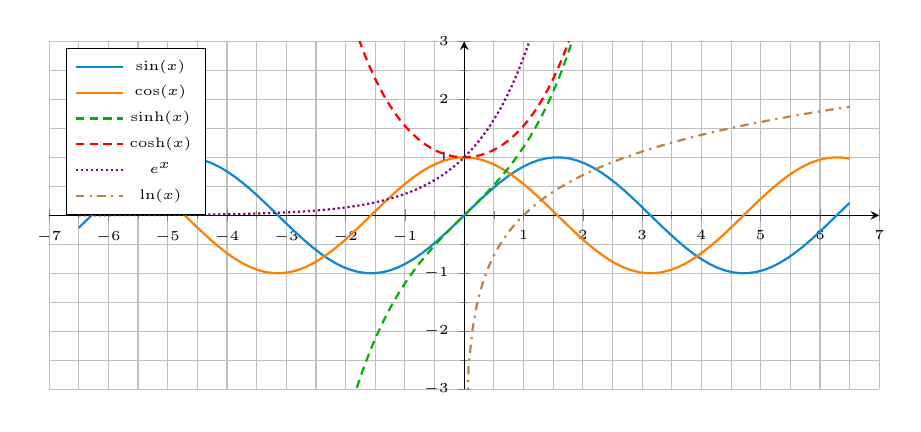
\begin{tikzpicture}
\begin{axis}[
    width=\linewidth,
    height=6cm,
    xmin=-7, xmax=7,
    ymin=-3, ymax=3,
    xtick={-7,-6,-5,-4,-3,-2,-1,0,1,2,3,4,5,6,7},
    ytick={-3,-2,-1,0,1,2,3},
    minor tick num=1,
    axis lines=center,
    grid=both,
    legend style={
        font=\tiny,
        at={(0.02,0.98)},
        anchor=north west
    },
    tick label style={font=\tiny},
    enlargelimits=false,
    samples=100
]
% sin(x)
\addplot [cyan!70!blue, thick, domain=-6.5:6.5] {sin(deg(x))};
\addlegendentry{$\sin(x)$}
% cos(x)
\addplot [orange, thick, domain=-6.5:6.5] {cos(deg(x))};
\addlegendentry{$\cos(x)$}
% sinh(x)
\addplot [green!70!black, thick, densely dashed, domain=-3:3] {sinh(x)};
\addlegendentry{$\sinh(x)$}
% cosh(x)
\addplot [red, thick, densely dashed, domain=-3:3] {cosh(x)};
\addlegendentry{$\cosh(x)$}
% e^x
\addplot [violet, thick, densely dotted, domain=-6.5:3] {exp(x)};
\addlegendentry{$e^x$}
% ln(x)
\addplot [brown, thick, dashdotted, domain=0.01:6.5] {ln(x)};
\addlegendentry{$\ln(x)$}

\end{axis}
\end{tikzpicture}
\end{center}

